\chapter{Results and analysis}
\label{ch:results}

From the experiments of the three architectures: Adversarial Anomaly Detector, sVAE, and GM-VAE; the one that presented the best reconstruction in the Adversarial Anomaly Detector (see figures \ref{fig:anogan_rec}, \ref{fig:svae_rec} and \ref{fig:gmvae_rec}). For the cases of both autoencoders, the reconstructions suffer from lots of blurring making difficult to evaluate the presence of an anomaly and hence confirming one of the main problems this kind of autoencoders. The problems in the autoencoders could the provoked for the series of gaps the learned data distribution has due to the initial assumption of make use of simpler data distributions as a base.

\begin{figure}[H]
\begin{minipage}{\linewidth}
  \centering
  \begin{tabular}{ccc}
  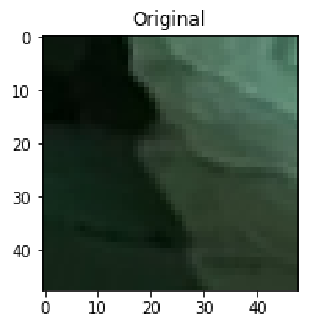
\includegraphics[width=.26\linewidth]{anogan_sample1_original}
    & 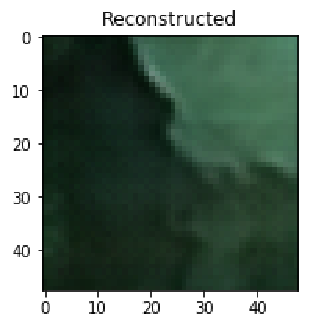
\includegraphics[width=.26\linewidth]{anogan_sample1_reconstruction} \\
  (a) & (b) \\
  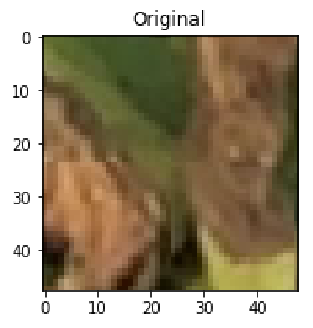
\includegraphics[width=.26\linewidth]{anogan_sample2_original}
    & 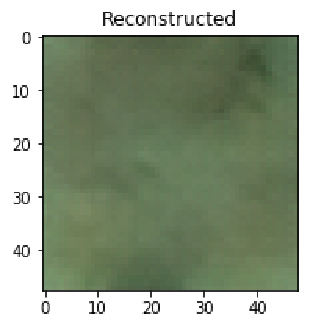
\includegraphics[width=.26\linewidth]{anogan_sample2_reconstruction} \\
  (c) & (d)
  \end{tabular}
  \end{minipage}
\caption[Reconstruction evaluation of the adversarial anomaly detector]{Reconstruction evaluation of the adversarial anomaly detector: a) origianl healty sample, b) reconstructed healty sample, c) original test sample and d) reconstructed test sample.}
\label{fig:anogan_rec}
\end{figure}

\begin{figure}[H]
\begin{minipage}{\linewidth}
  \centering
  \begin{tabular}{ccc}
  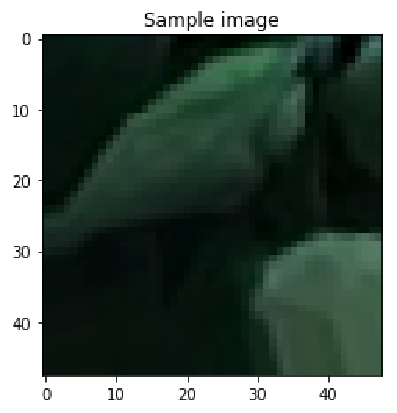
\includegraphics[width=.26\linewidth]{svae_sample1_original}
    & 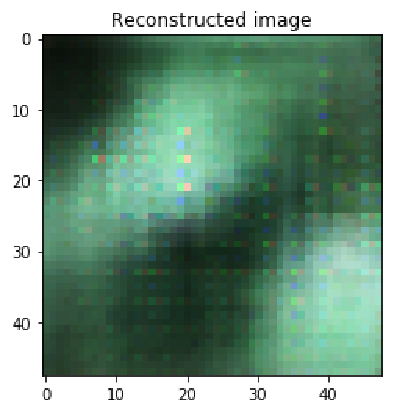
\includegraphics[width=.26\linewidth]{svae_sample1_reconstruction} \\
  (a) & (b) \\
  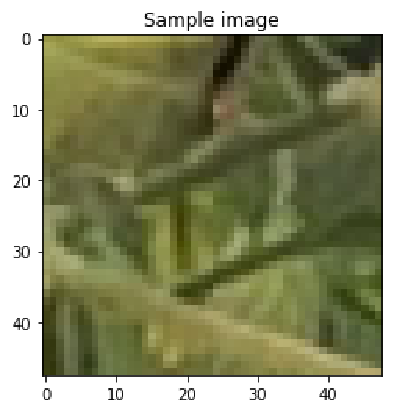
\includegraphics[width=.26\linewidth]{svae_sample2_original}
    & 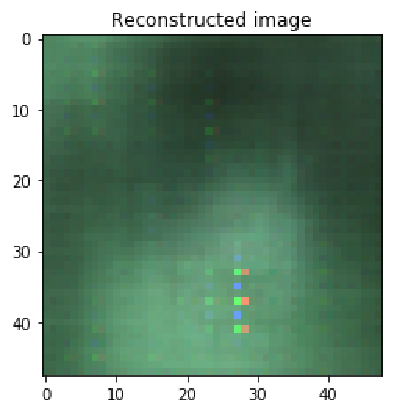
\includegraphics[width=.26\linewidth]{svae_sample2_reconstruction} \\
  (c) & (d)
  \end{tabular}
  \end{minipage}
\caption[Reconstruction evaluation of the sVAE]{Reconstruction evaluation of the sVAE: a) origianl healty sample, b) reconstructed healty sample, c) original test sample and d) reconstructed test sample.}
\label{fig:svae_rec}
\end{figure}

\begin{figure}[H]
\begin{minipage}{\linewidth}
  \centering
  \begin{tabular}{ccc}
  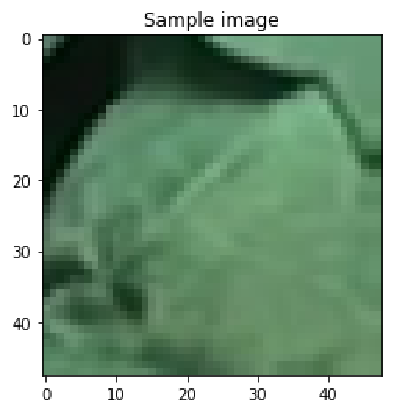
\includegraphics[width=.26\linewidth]{gmvae_sample1_original}
    & 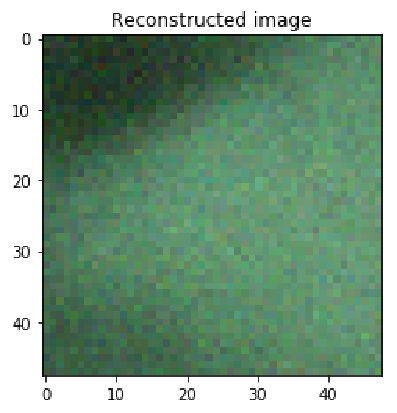
\includegraphics[width=.26\linewidth]{gmvae_sample1_reconstruction} \\
  (a) & (b) \\
  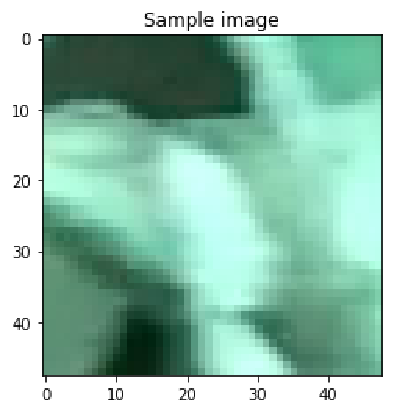
\includegraphics[width=.26\linewidth]{gmvae_sample2_original}
    & 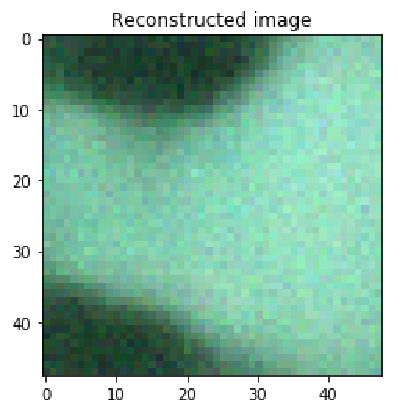
\includegraphics[width=.26\linewidth]{gmvae_sample2_reconstruction} \\
  (c) & (d)
  \end{tabular}
  \end{minipage}
\caption[Reconstruction evaluation of the GM-VAE]{Reconstruction evaluation of the GM-VAE: a) origianl healty sample, b) reconstructed healty sample, c) original test sample and d) reconstructed test sample.}
\label{fig:gmvae_rec}
\end{figure}

In the case of the AnoGAN, one of the more problematics parts was the training of the model, but with the available tomato date, it was possible to achieve the Nash equilibrium. The generated images are much better than the ones in the autoencoders. Its main disadvantage is the time needed to learn a set of latent variables to reconstruct some images. This problem is resolve with the introduction of an encoder in the AnoGAN architecture as shown in the table \ref{table:rec_time}.

\begin{table}[htb]
    \caption[Reconstruction time evaluation]{Reconstruction time evaluation.}
    \label{table:rec_time}
    \centering
    \begin{tabular}{ c c c }
        \hline
        Model & Reconstruction time (ms) \\
        \hline
        sVAE & 160.8 \\
        GM-VAE & 1383.1 \\
        AnoGAN & 6320.6 \\
        Adversarial Anomaly Detector & 255.3 \\
        \hline
    \end{tabular}
\end{table}

In figures \ref{fig:anogan_eval_test_image_1} and \ref{fig:anogan_eval_test_image_2} is possible to see the data distribution between normal and anomaly samples. For the case of the figure \ref{fig:anogan_eval_test_image_1} we can see a defined group of data that represents the healthy samples and a smaller amount of points around this healthy group that represents the anomaly data. In the figure \ref{fig:anogan_eval_test_image_2} we have the opposite case, where the amount of anomalies is bigger than the number of healthy samples.

\begin{figure}[htb]
  \centering
  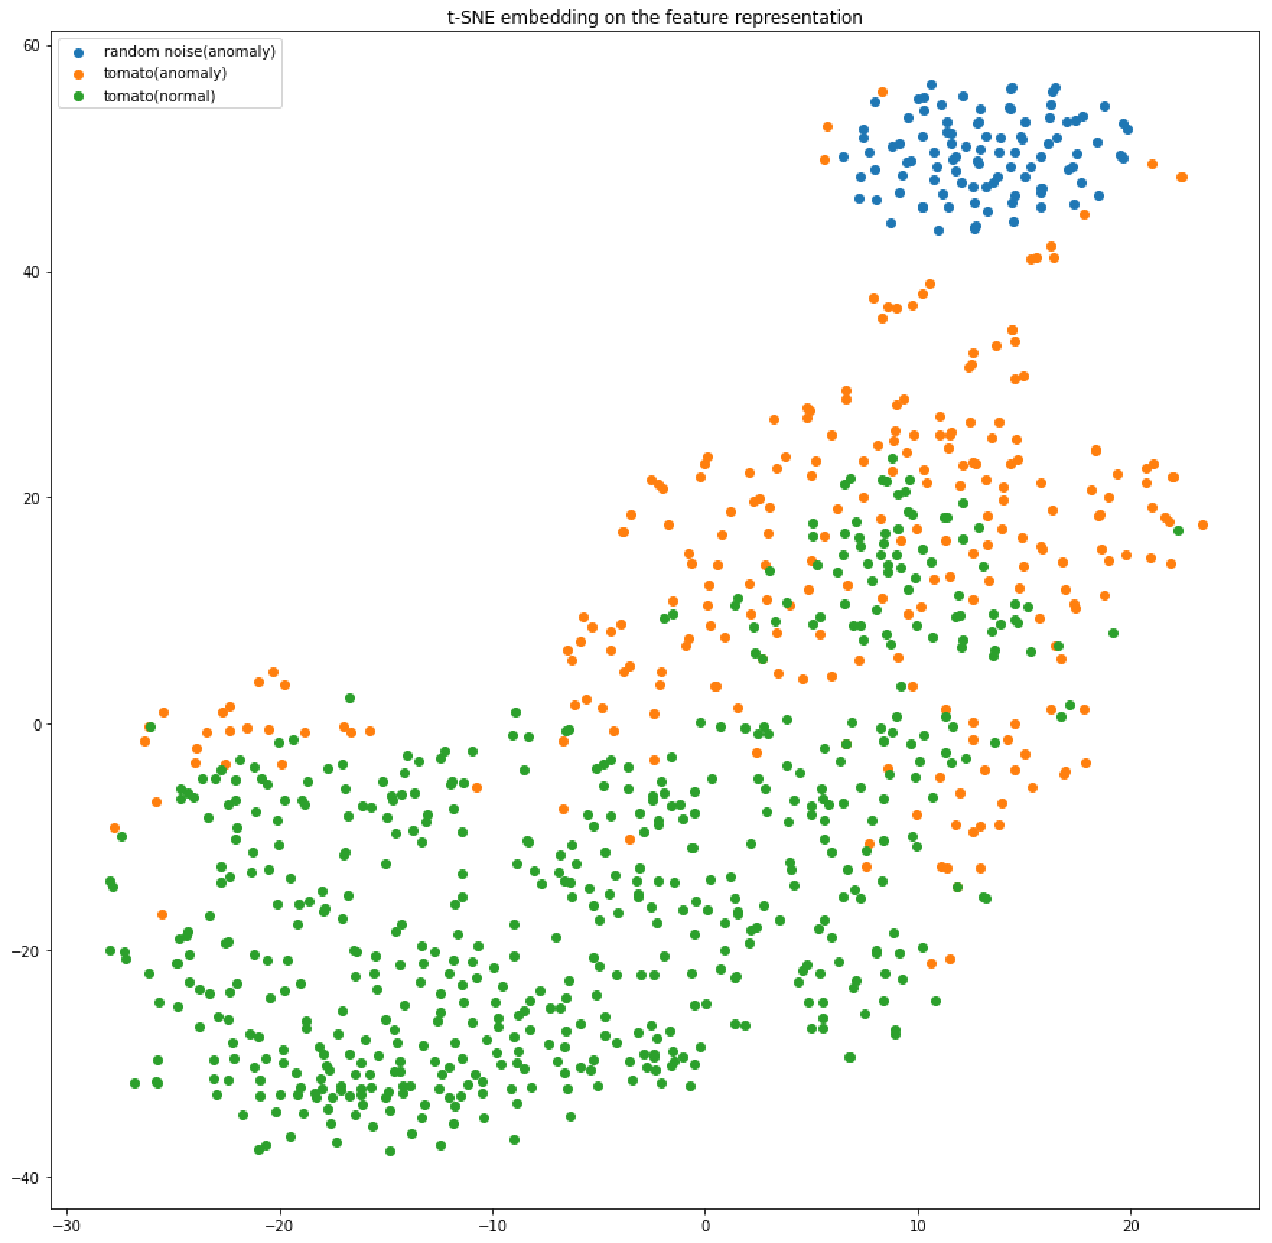
\includegraphics[width=150mm]{anogan_t_sne1}
  \caption[Adversarial Anomaly Detector t-SNE evaluation of test image 1]{Adversarial Anomaly Detector t-SNE evaluation of test image 1}
  \label{fig:anogan_eval_test_image_1}
\end{figure}

\begin{figure}[htb]
  \centering
  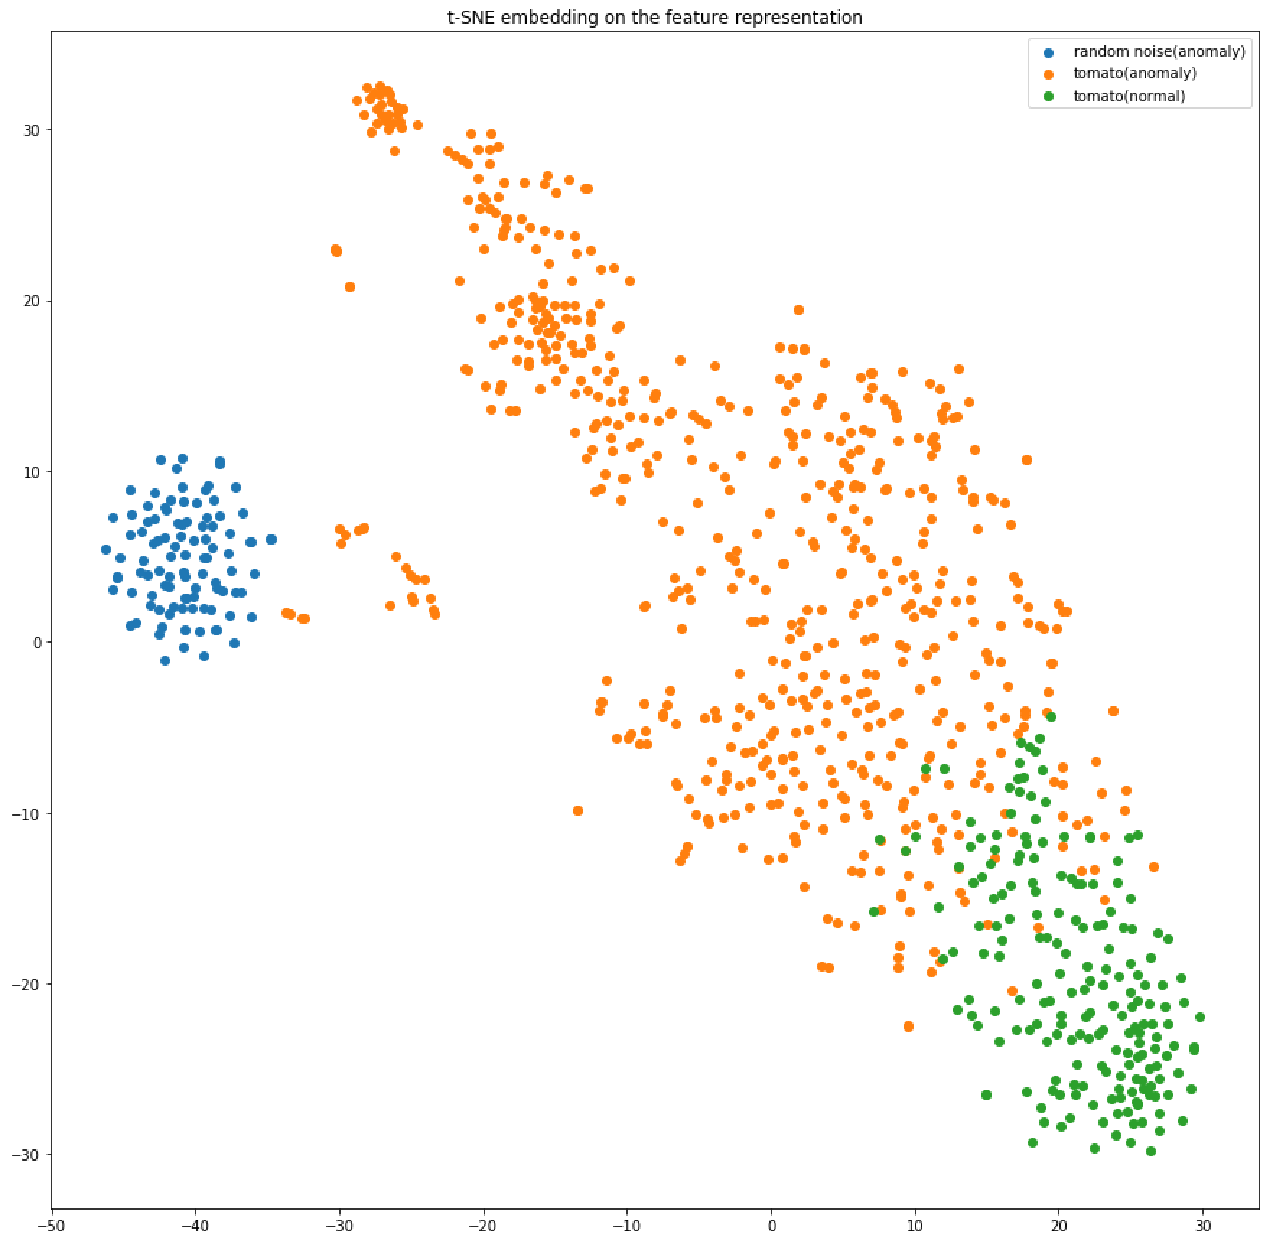
\includegraphics[width=150mm]{anogan_t_sne2}
  \caption[Adversarial Anomaly Detector t-SNE evaluation of test image 2]{Adversarial Anomaly Detector t-SNE evaluation of test image 2}
  \label{fig:anogan_eval_test_image_2}
\end{figure}
